% Created 2019-07-03 Wed 00:06
% Intended LaTeX compiler: pdflatex
\documentclass[11pt]{article}
\usepackage[utf8]{inputenc}
\usepackage[T1]{fontenc}
\usepackage{graphicx}
\usepackage{grffile}
\usepackage{longtable}
\usepackage{wrapfig}
\usepackage{rotating}
\usepackage[normalem]{ulem}
\usepackage{amsmath}
\usepackage{textcomp}
\usepackage{amssymb}
\usepackage{capt-of}
\usepackage{hyperref}
\usepackage{minted}
\author{Nicolás Luarte}
\date{\today}
\title{Cynthia}
\hypersetup{
 pdfauthor={Nicolás Luarte},
 pdftitle={Cynthia},
 pdfkeywords={},
 pdfsubject={},
 pdfcreator={Emacs 25.2.2 (Org mode 9.2.3)}, 
 pdflang={English}}
\begin{document}

\maketitle
\tableofcontents

\section{Ciclos}
\label{sec:org70f7062}
\begin{center}
\begin{tabular}{lll}
Ejercicio & Protocolo & Bloque\\
\hline
Sentadilla de competencia & x6@8, 15\%, 4x7 & A\\
Sentadilla de competencia con pausa (3 ct) & x6@8, 15\%, 2x6 & A\\
Banca de competencia & x4@8, 10\%, 4x6 & A\\
Banca de competencia con pausa (5 ct) & x2@8, 15\%, 4x3 & A\\
\hline
Banca agarre cerrado & x8@8, 10\%, 3x8 & B\\
Peso muerto de competencia (sumo) & x5@8, 15\%, 3x5 & B\\
Peso muerto hasta las rodillas & x7@8, 15\%, 2x7 & B\\
Peso muerto bloques (abajo de las rodillas) & x10@8, 10\%, 2x10 & B\\
\end{tabular}
\end{center}
\section{Comentarios técnicos}
\label{sec:org42740cb}
\section{Registro de progreso}
\label{sec:orgb0b5249}
\begin{center}
\label{tab:org9c541b6}
\begin{tabular}{llll}
Ejercicio & RPE & Peso & Fecha\\
\hline
 &  &  & \\
\end{tabular}
\end{center}
\begin{center}
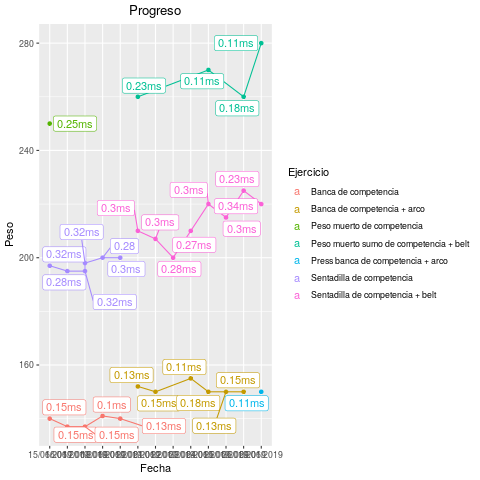
\includegraphics[width=.9\linewidth]{tmp.png}
\end{center}

\section{Tiempo de peak}
\label{sec:orgd953ccb}
5 exposiciones
\end{document}
